\begin{comment}
Things to get into this section
%===============================

FDA 15	Hotelling / Palander competition dynamics
WUD 16	Hotelling Palander model: simple example for blind agents finding trade-off optima?
Note: this is shorn of all space costs. It's just about the effect of spatial competition. 

WUD 19	Value density: a natural idea from combining utility with Weber-like analysis, and also useful in the real world. Cf. Isard; certain things can be given infinite weight; cf. Storper and trade costs: human-capital intensive = humans are heavy!

WUD 22	Transport intensity: as a concept, need tangled bank?

WUD 22	Externalities, ubiquities, central places, density maps, discrete spatial choices

WUD 22	"CES, supermarkets": explain through love of variety while minimising space/information costs.

%WUD 27	Here and not-here: can be defined with externalities as well as transport costs.

WUD  28-9	Krugman's intermediates. Krugman (and later theorists) are arguing this CES approach to intermediates negates the need for thinking about 'Weber-type problems', and provides a clearer answer.

WUD 31	Such a thing as cost proximity? i.e. distance = further, overall cost = less? Does this mean space can be considered just another factor after all?

WUD 34	What's the difference between a worker and an order of steel? The steel doesn't need to go home and sleep every night. Labour as a factor is unique, and relates to space and time in a particular way. 
Cf.2 migration and commute.

Other random things:

1d vs d2: chapman's intervening opportunities example, and that one paper that looks at the same problem. You know the one! Anyway, they're both in the spacecostswriteup table.

\end{comment}

\section{Key space concepts \label{sec:spaceconceptsintro}}

%===============================

\subsection{Spacey spacey \label{sec:spaceyspacey}}

%WUD 45	Line for intro: : how has space been theorised? All the way from "just a cost" - Predohl's reducing it to price, right through to the most detailed.

This section explains how the theorisation of space has been used to develop the model philosophy of the thesis. Using Isard's ideas from the introduction to this section, two extreme poles of spatial theorisation can be defined: `implicit' versus `explicit'. At the implicit end, space does not matter: distance is reduced to a simple cost, no different to any other. At the opposite pole, space enters entirely explicitly into models: actors have locations, and space itself can be an agent, able to impact on actor outcomes.

%WUD 9	Fujita quoting Isard talking about Chamberlin! The latter: space is just another vector of product differentiation. (p.377) WUD 9	Fujita: multiple solutions, from endog agglom leading to lock-in, meaning indeterminacy.
At the extreme implicit end, the obvious economic approach is to treat the effect of distance as just another cost, integrated into the price system. Isard notes how one theorist (Pred\"{o}hl) ``wished to investigate how far the location problem is a price problem; location theory, a price theory. In other words, to what extent does the local distribution of production lie inside the economic relationship of interdependent prices?'' (\citealt{isard_location_1956} p.483) Fujita points out that Chamberlin believed space to be just another vector of product differentiation (\citealt{fujita_location_1999} p.377). If it could be made to do so, then space is not a unique factor - and does not affect the assumptions necessary for a perfect competition market structure.

Right at the other end, there is the `Weberian' approach: as Alfred Weber does, this allows economic actors explicit spatial coordinates, which enter into their calculations when finding optimum outcomes (\citealt{weber_theory_1909}). Added to this, raw distance can then have a cost, which can be affected by other factors such as weight. This level of explicit space is entirely within reach of agent models, but is it a useful thing to do? Isard, for one, saw the value of avoiding the ``necessity of tagging each unit of land, labour and capital with a set of absolute spatial co-ordinates'' (\citealt{isard_location_1956} p.36). One might respond, he didn't have access to computers. It will be argued below, however, that continuous, explicit space has both positive and negative implications for spatial economic modelling.

All of the model runs in this thesis use some form of explicit space. This excludes `Thunen'-like space used in urban economics, which is continuous but analytic, containing no explicit location, and using a `spatial equilibrium' where utility is presumed \emph{a priori} to be identical for all actors (see e.g. \citealt{glaeser_cities_2008} pp.19). The discrete-region models of \gls{ge} theorise space in a particular way; this is discussed in section \ref{sec:keyconcepts_coremodel} in more depth, but the key modelling point is that the approach is easily subsumed into a framework that includes continuous space. 

%%%%%%%%%%%%%%
% TYPES OF SPACE USED WOZ ERE
%%%%%%%%%%%%%

%The argument developed in this section is that choice of space-type affects model outcome, and that assumptions made in one are often null in others. 
As mentioned in the introduction to this chapter, `Weber-type' stories are dismissed by Krugman and discounted by Fujita \emph{et al} (\citealt{fujita_spatial_2001} p.26) as only relevant to `optimal plant location' considerations. Industrial location theory is partial, of course, so it might seem reasonable for theorists chasing generality and endogenous outcomes to dismiss it. Yet Isard - the first to attempt a `general location theory' - argued that Weber succeeds in developing a theory able to capture the prime empirical fact of distance. His own early work on the coal and steel industry (\citealt{isard_locational_1948}) is, perhaps, just the sort of 'Weber-type story' that Krugman refers to: it lays out the historical detail of a shift in the balance of forces between inputs and market location, with little reference to any micro-economic underpinning. 

This is not because Isard thinks the economics are unimportant; rather, he sees a role for `supplementary' theories capable of working better with the central empirical facts about the `distance factor', in contrast to formal theory which, by itself, is ``too general and too sterile.'' (\citealt{isard_location_1956} p.36}) The job of the upcoming section is to identify the ways in which different types of spaces may affect model outcome. Later chapters will then examine whether agent modelling can achieve a different approach to the sort of explicit-space analysis Isard thought worthwhile. The next section starts by returning to externalities. 
\cmt{summarise final structure of space concepts section when finished}

%%%%%%%%%%%%%%%%%%%%%%%%%
% EXTERNALITIES IN SPACE
%%%%%%%%%%%%%%%%%%%%%%%%%
\subsection{Externalities in space \label{sec:extsinspace}}

Section \ref{sec:externalities} explained that externalities can be defined by introducing external values directly into an actors' utility or production function, or introducing them after these - for example, into a firm's profit level. Spatially, this works simplest if discrete regions are used (though there are continuous space options; see below). With a discrete space-type, external economies are easily implemented. For instance, in a two-region model with regions $r$ and $s$, firms in $r$ could include in their production function the total output of other firms in that region, $nx$. Using Scitovsky's way of defining an externality, that would be:

\begin{equation}
x_{r}=F(l_{1},c_{1},...;nx)\label{eq:locext1}
\end{equation}

This is a `localisation externality': an effect that stems from being `here'; as such, it relies on `here' being a discrete place. In Scitovsky's terms, the above is also a pure externality since it enters directly into the production function. Economically, what does it mean? The classic example goes back to Marshall: the number of firms of the same industry increases the stock of knowledge for all firms in that region. This is often defined in terms of the number of workers in a region also; their presence acts as a knowledge multiplier as they move between firms. 

These `Marshall externalities' are often contrasted to `Jacobs externalities'. These attempt to capture the central thrust of Jane Jacobs' argument: that diversity of production lies at the heart of regional productivity. A simple way of achieving this would be to insert a CES-type function into \ref{eq:locext1} rather than the raw number of firms: a region's productivity could thus, in effect, have a `love of variety'. (Jacobs' ideas will be discussed in more depth in chapter \ref{chapter:ABM}, where this simple approach to her diversity argument will be questioned.)
\cmt{examples from literature plz!}

Using localisation externalities in discrete regions has clear advantages. The effect of proximity is definable in a tidy way; they are either inside an actors' production or utility function, or they are not. One of the clearest benefits of this is empirical comparability. Being able to define a direct mathematical relationship between regional output or diversity and overall firm levels gives a simple route to regression analysis - a fact used by Glaeser \emph{et al} (\citealt{glaeser_growth_1992}) to identify Jacobs externalities as the most powerful (a result since challenged by e.g. \citealt{van_der_panne_agglomeration_2004}).

But are there any downsides in reducing space effects to nothing more than the difference between `here' and 'elsewhere'? One approach is to combine an element of space cost with externalities: the \gls{coremodel} does this, as discussed more below. Raw distance, still, is clearly important. Black and Henderson (\citeyear{black_spatial_1999}, p.327) point out what might appear a very obvious possibility: ``capital good plants agglomerate in locations with high manufacturing employment even though this generates no externalities: it just conserves on transport costs of exchange.'' Does the discrete externality approach hide this, or can it account for it? The next section compares these externalities to the idea of `agglomeration' to start answering this question.
\cmt{Still a little bit too whodunnit... and do I answer the question?}

%WUD 33	Some notes on externalities; there's a point there but can't quite nail it down currently. I think it's important though. Might be some good medium-complexity model atoms here.

%WUD 46	When every agents' movement affects every others' outcome, is it useful to treat it as an externality? Cf. Scitovsky's point about pecuniary externalities: what distinguishes them from normal price signals? 
%How to define externalities when there's no simultaneous calculation? Over time - cf above - doesn't it just work out as part of the price system?
%Externality: an "outside price system" effect.


%%%%%%%%%%%%%%%%%%%%%%%%%%%%%%%%%%
% AGGLOMERATION AND 1ST/2ND NATURE
%%%%%%%%%%%%%%%%%%%%%%%%%%%%%%%%%%

\subsection{Agglomeration and `first versus second nature' effects \label{sec:agglom}}

In this thesis, agglomeration is separated analytically from agglomeration \emph{effects}. It is used as a verb: agglomeration is a process, rather than a synonym for `city' or `centre'. In discrete space, agglomeration occurs simply when agents move into a region: it can be measured straightforwardly by the change in regional totals. If they move there because of some regional externality caused by agent numbers, that is an agglomeration \emph{effect}. In continuous space, the definition has to be a little more convoluted, though the intuition is straightforward: agglomeration and clustering are the same. All agents have point locations, and so a point cluster measure can be used. The simplest way of doing this is to use `actor-wise' mean nearest neighbour distance: distance to neighbours can be summed and averaged for each actor. These values can then be averaged again over \emph{all} actors to produce an aggregate figure. Statically, this is little use, but differenced over timesteps, this can give an aggregate measure of agglomeration change. How this changes between timesteps measures agglomeration change. (See figure \ref{fig:agglomex} for an example in $R^2$, which shows agglomeration taking place initially, with a burst of dispersion towards the end of the model run.)

%C:\Users\Dan\Dropbox\java\backyard2\data\25.7.10.400peep4dayrad2
\begin{figure}%
\centering
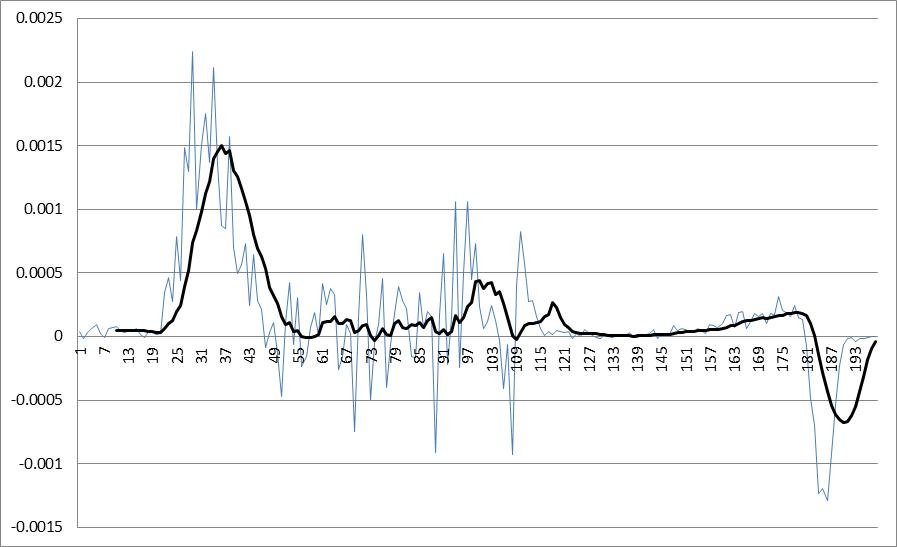
\includegraphics[width=0.5\columnwidth]{ChapterEcon/figures/exampleagglom}%
\caption{Example of agglomeration over time, measured with mean nearest neighbour distance.}%
\label{fig:agglomex}%
\end{figure}

So, as regards the discussion of localisation externalities above: these are agglomeration effects (sometimes described in the literature as `localisation externalities' or `localisation economies'; e.g. \citealt{malmberg_elusive_2002}, \citealt{wheeler_localization_2007}, \citealt{figueiredo_localization_2009}). Glaeser talks of `agglomeration economies' that ``exist whenever people become more productive through proximity to others'' (\citealt{glaeser_cities_2008} p.5). Again, by the definition used here, these are agglomeration effects. 

%There are many different terms for the opposite of agglomeration: classically, Weber used `deglomeration' (\citealt{weber_theory_1909}); Krugman uses centrifugal forces, opposed to centripetal forces holding places together; Brakman et al use `spreading'. This thesis will use dispersion, following Fujita and Thisse (\citealt{fujita_agglomeration_2002}), and again, this is a  measureable output of the model.

%cut and paste from intro. 
%cf Fujita: WUD 9	``To test whether a...
%note this Krugman paper I iz not red: Krugman, Paul R. 1993b. First nature, second nature, and metropolitan location. Journal of RegionalScience 33(2):129�144.
%-  empirically it has been shown that 1st nature effects can account for only about 20\% of the observed location patterns. \fixref{citations for 1st/2nd n} Glaeser et al, which paper? And Jacobs.}
\gls{ge} wants to explain agglomeration ``as an endogenous outcome of the economic process'' (\citealt{storper_agglomeration_2010}, p.315), which is to say that `first nature' effects - location being determined by natural harbours or resource availability, for example - are considered uninteresting. Their role is acknowledged, but the goal is to identify and understand `second nature' effects - those that flow from the interaction of people and firms alone. As Glaeser argues (\citealt{glaeser_cities_2004}, \citealt{glaeser_cities_2008} p.7), the decline in transport costs emphasises second nature, endogenous sources of agglomeration because the importance of absolute location declines along with those costs. On this basis, Fujita argues that - 

\begin{quote}
``To test whether a model can explain the endogenous formation of agglomerations, it is best to consider the simplest case of a perfectly homogenous geographical space (and free choice of location by all agents), for if any concentration of economic activities occurs in such a homogenous space, it must be due to endogenous forces of agglomeration.'' (376-7)
\end{quote}

\gls{ge} modellers are thus suspicious of any theory that supplies exogenous difference to start with, such as trade models based on factor differences. It is straightforward enough to identify some first nature effects; for example, Storper (\citeyear{storper_agglomeration_2010} p.316) identifies ``propulsive activities such as political power (the State), trade (rivers and ports), and finance''. The difference between these and second nature, however, breaks down in models running over several timesteps. Analytically, first and second nature effects can be distinguished thus: first nature geography is determined by absolute location (such as a resource site or port), second nature by relative location - that is, the effect comes about through interaction between locations. But as O'Sullivan and Unwin point out, ``it is usually impossible to distinguish these effects in practice simply by observing the intensity of a process as it varies across space.'' (\citealt{osullivan_geographic_2002}, p.79) 

A stronger argument than this can be made: the one necessarily leads to the other. In section \ref{sec:backyard}, the simplest model of agglomeration in $R^2$, as soon as two actors have formed a collaboration, they become a first-nature effect: their absolute location determines subsequent timesteps. One obvious conclusion: it is possible to have endogenous first nature effects. In an agent model, the actual location of those first nature effects will vary entirely normally as the random seed of the model is changed. Section \ref{sec:keyconcepts_coremodel} points out the importance of cumulative causation for \gls{ge}, but this somehow seems to focus too heavily on the idea that second nature effects should be isolated. In an agent-based, iterative context, that is not possible. As will be argued, there is a related problem in defining externalities over several timesteps, for actors in continous space.

%WUD 21	Common def of 'localisation' actuall opposite to GE. Dispersion, move towards autarky.
%http://transitionculture.org/2010/07/30/localism-or-localisation-defining-our-terms/ Useful: so, I should be able to cite Hopkins.
As a final note for this subsection: a common meaning of the term `localisation' in the non-economic literature is actually opposite to how it is understood in \gls{ge}. Hopkins cites Shuman: ``It means becoming more self sufficient, and less dependent on imports.'' As Hopkins says, it is about ``building more localised economies''. In \gls{ge} terms, however, this is exactly the opposite: it is moving in the direction of autarky, where regions become less specialised. It is actually dispersion.
\fixref{localisation: Hopkins' dissertation}
%How would that compare with the distinction between localisation and urbanisation economies? Hmm...

%%%%%%%%%%%%%%%
% little cuttinz!
%%%%%%%%%%%%%%%
\begin{comment}
Proximity is 
Glaeser is rather less equivocal about the importance of proximity: 
\begin{quote}
``The benefit of being in a city is closeness to the other people in that city... Proximity reduces transport costs for goods, for people and for ideas.'' (\citealt{glaeser_cities_2008} p.117)
\end{quote}
For Glaeser, this basic fact about proximity gives a straightforward way to define agglomeration: ``agglomeration economies exist whenever people become more productive through proximity to others'' (ibid p.5). 

\begin{quote}
``The benefit of being in a city is closeness to the other people in that city... Proximity reduces transport costs for goods, for people and for ideas.'' (\citealt{glaeser_cities_2008} p.117)
\end{quote}
For Glaeser, this basic fact about proximity gives a straightforward way to define agglomeration: ``agglomeration economies exist whenever people become more productive through proximity to others'' (ibid p.5). 

I should define agglomeration, for my model. No reason why that can't happen there. Er. Noting that it's different for discrete regions and continuous spaces. The former is a very straightforward gravity-model approach, used even by GE. The latter, I am defining as change in mean nearest neighbour distance over time. That makes it separate from agglomeration effects - which are really 1st nature effects in continuous space. (Because analytically you can't tell them from any other; e.g. backyard: one small seed of agglomeration becomes as much a 1st nature effect as a port.)
%``Urban centres came into existence because they concentrated 
\end{comment}

%%%%%%%%%%%%%%%%%%%%%%%%%%%%
% MARKET STRUCTURE AND SPACE
%%%%%%%%%%%%%%%%%%%%%%%%%%%%
\subsection{Market structure and space \label{sec:marketstructnspace}}

%WUD 44	think I need some very simple math examples for:
%http://www.kgbanswers.com/is-nix-a-word/4042728 Is nix a word? Yes!
Why has market structure been such a sticking point for spatial economic modelling? A short summary goes like this. Perfect competition cannot work with increasing returns, because any firm able to gain them will have a cost advantage: that is immediately no longer perfect competition. It would also nix the possibility of assuming agents are price-takers and that there is one price. (This was covered in section \ref{sec:marketstructure}.) Economics in space, however, cannot work \emph{without} increasing returns, because if output in linear, gains from trading across space can never be enough to compensate for losses incurred transporting goods or people. 
%Though note: those inc rets could be either productive or utility / love of variety, and like the cobb douglas, they would actually look the same!)
%Also, is that true if linear output is heterogenous? E.g. comparative advantage.

As discussed, this issue led to space being largely ignored by mainstream economics. As Fujita put it:

%WUD 9	Fujita: 
\begin{quote}
``since the traditional general equilibrium analysis abstains from the consideration of indivisibilities or increasing returns, it fails to capture the essential impact of transport and spatial costs on the distribution of economic activities.'' (\citealt{fujita_location_1999} p.376})
\end{quote}

The way in which perfect competition rules out spatial economic models has been dubbed the `spatial impossibility theorem' by Fujita. Starrett (1978) is credited with first making this point formally. As Fujita and Thisse describe it -

%''The essential question is whether the competitive price mechanism is able to explain the endogenous formation of economic agglomerations. To check the ability of a spatial model to do so, the best approach is to consider the case of a homogenous space in which economic agents are free to choose their locations...'' 
\begin{quote}
``Starrett has shown that if space is homogenous and transport costly, then... the economy degenerates into separate single-location groups of agents with all trades taking place within, rather than between, groups. Consequently, the perfectly competitive price mechanism alone is unable to deal simultaneously with cities and trade.'' (\citealt{fujita_economics_2002} p.13-14) 
\end{quote}

To put it another way: if an actor is able to produce `in their own backyard', why would they choose to trade or collaborate in a world where all producers' output is linear? Any gain they would receive can never outweigh transport costs, if output in linear. However, with increasing returns introduced to the picture, the minimum conditions for spatial economic activity now exist. (This `minimum condition for agglomeration' is investigated in more detail through the models in section \ref{sec:backyard}.)

So increasing returns serve a dual purpose: as discussed in section \ref{sec:marketstructure}, they guarantee uniqueness of varieties so no single monopolist can emerge. They also allow actors to break out of this `spatial impossibility' trap. This dual purpose, however, hides an effect that comes from the type of space used. The CES approach used in \gls{ge}, built on the \gls{dxs}, guarantees a diversity of firms. As will be shown in chapter \ref{chapter:models} in detail, however, space itself can provide that diversity in a two-good model where, in discrete space alone, such a limited number of goods would lead to problems. The basic issue is that several firms competing on a single point, selling the same good, find themselves in a \gls{bertcomp} situation: lowering their price by a tiny amount will result in taking the entire market, where consumers are all on the same spot. The analytic, rational result is for firms to set price at marginal cost (see e.g. \citealt{varian_intermediate_2006} p.495). In an increasing returns situation, however, the result will be that if one firm gets a toe-hold in cheaper production, cumulative causation leads to monopoly.

That space itself offers this resistance to extreme dynamics is not a new point; again, it is something Isard discusses. Space guarantees market areas overlap and immobilities exist; for this reason alone, Isard argues, ``the generally accepted principle of pure competition is not applicable to the analysis of spatial economic processes.'' (489-490) Note, however, this is a different argument to `incomplete competition' due to increasing returns or spatial impossibility. Isard is talking about something much more basic: space itself imposes those limitations. As the model results will show, this is born out by the effect space-type has on outcomes.

%It is worth noting that, historically, `backyard' production of various sorts has been a commonplace. Sheffield cutlers, for example, worked in this way, with many homes having their own mini-forges. \cmt{Sheffield cutlers? Citation?} 
%Bertrand paradox; CES needed to avoid monopoly in discrete regions; not needed in 2D continuous space. MM2 50	Does R2, by default, break out of Bertrand's paradox? (Cf. Bertrand's paradox and differentiation.) Cf. http://en.wikipedia.org/wiki/Bertrand_competition
%"Well, having just run another Torus model, I realise that space - introducing differentiation as it does - solves many of the problems inherent in point-economies, and does away with the analytic need for a product differentiation function like the CES for avoiding monopoly." (fielddiaryAutum2010 p.18)
%FDA 17	Avoiding total monopoly on a point: CES and monocomp. Avoiding monopoly in the real world: 2D space. Cf. Isard on overlapping markets.
%Or p.18: continuous space - introducing differentiation as it does - solves many of the problems inherent in point-economies, and does away with the analytic need for a product differentiation function like the CES.

%%%%%%%%%%%%%%%%%%%%%%%%%
% CORE MODEL KEY CONCEPTS
%%%%%%%%%%%%%%%%%%%%%%%%%
\subsection{Key concepts from the core model \label{sec:keyconcepts_coremodel}}

There are two good reasons for looking at Krugman's original \gls{coremodel}. Firstly, it can serve as a useful way for understanding how space has been theorised in \gls{ge}. Later, in chapter \ref{chapter:ABM}, the work of Christopher Fowler on creating an \gls{abm} version of Krugman's model will be a useful jumping off point for explaining the approach taken in this thesis. Secondly, it presents ample opportunity for exploring how a now well-developed, but relatively new, approach has dealt with the `realism versus relevance' debate. It is particularly good for this since the issues have been openly discussed. 

\cmt{first mention of the realism versus relevance debate? If so, needs mentioning in intro. Full section is in ch.4}

It is not necessary to outline the full details of the model here; Brakman \emph{et al} and Fowler are both good places to get these. Appendix \ref{apx:maths} gives an explanation of the model sufficient for getting a simulation up and running and understanding the results, and discusses some model nuts and bolts further. The task of this section is pull out those features of relevance to understanding the key space concepts. 
%Krugman's original \gls{coremodel} illustrates all the principles of \gls{ge}. This section pulls out the relevant key concepts. Section \ref{coremodelapx} of the mathematical appendix has more detail on the structure of the core model, but it is kept out of here to keep a focus on those aspects of direct interest for the thesis.

The core model wants to do for geography what Krugman's trade theory did for models of international trade: explain how the trade patterns seen in the real world can come about with no fundamental initial differences - just slight differences in initial conditions determining which places are core, which periphery. Cumulative causation then leads to equilbrium outcomes. This is far from being a new idea, of course: Chapman describes Myrdal (1957) arguing that ``the mechanisms of cumulative causation inevitably tend to accentuate economic inequalities between regions leading to the emergence of a dynamic core surrounded by a stagnant or declining periphery'' (\citealt{chapman_people_1979} p.92). Krugman's stated aim was to formalise this in an equilibrium setting.

The \gls{coremodel} examines the interaction between a direct `transport cost' and externalities to make its case. Transport costs are defined between regions; these costs enter directly into the model's functions. In theory (see below), actors are also affected by externalities within regions: the number of workers in one region affects the total number of firms there. 

The \gls{coremodel} has two `moments' of time. The initial short run (found by a brute-force solving of the set of simultaneous equations outlined in table \ref{tab:op_eqs_coremodel}) gives the real wage for two regions. Depending on the initial conditions, these will be higher in one region than the other. The model's second moment might be considered a second externality, as the wage level in the opposite region enters into workers' location choice. This is argued to be a natural consequence of the difference in real wages found initially: these will equilibriate as workers move region, at a rate proportional to the difference between the two regions (see \citealt{fowler_taking_2007} pp.270 for a clear outline of this.) 

%requires a separate argument. In the first, each region has its own set of simultaneous equations (See table \ref{tab:op_eqs_coremodel}) containing both regions, the real wage, the price index and regional income. 
To achieve this, the two `moments' consist firstly of a set of simultaneous equations, followed by something akin to a gravity model to do the job of finding the equilibrium level of workers. Brakman \emph{et al} suggest there are:

\begin{quote}
``four different economic agents in the core model... namely the manufacturing workers in both regions, and the farmers in both regions. This reduces to three economic agents in the long-run equilibrium, in which the real wage is the same for all manufacturing workers.'' (\citealt{brakman_new_2009} p.128)
\end{quote}

In terms of the actual equation structure, however, the two sectors of workers are combined in one income level per region. This is a \gls{repag}, standing in for the actions of all actors in that region. (See section \ref{sec:micromacro} for a full discussion of this.) The migration of manufacturing workers is the heart of the model; the existence, number and location of firms is deduced from this movement. `Agricultural worker' agents have a dual purpose: to provide a positive demand for both regions (since they cannot migrate) and to act as the base of comparison for model change. They do this by providing the numeraire: agricultural output is linear, and the number of agricultural workers is fixed, so the value and quantity of this output does not change. Demand does not change for agricultural goods as other workers migrate, as they are exempted from transport costs; in effect, all agricultural produce is available from a single market across both regions. In practice, what this means is that the number of agricultural workers can stand in as agricultural income in the final equations (again, see table \ref{tab:op_eqs_coremodel}).
\cmt{first mention of numeraire? Needs to be in econ concepts.}

The `two goods' model discussion in section \ref{sec:twogoodsmodels}\cmt{two goods ref, will change} talks more about the problems of translating the numeraire approach into an agent context. In searching for a base for comparison, the \gls{coremodel} offers another idea: one can ask, ``what is the minimum amount of expenditure required to buy one unit of utility?'' (\citealt{brakman_new_2009} p.99) In the models here, `expenditure' at base is time, so the question for actors becomes, `can I get more utility for my time?' This is used to help explain the model framework in section \ref{sec:turntimetoutil}.

As pointed out in section \ref{sec:extsinspace}, space costs enter into the \gls{coremodel} in two ways. There is an explicit space cost for manufacturing goods to move between regions, and there are externalities: the discrete effect of being `here'. As well as externalities stemming from worker numbers (and thus firm numbers since, in the \gls{coremodel}, one implies the other), there is the `second moment' argument made about worker migration. While this migration can be framed as an externality, actual movement is costless - and since the location of firms is just the mirror of manufacturing workers' location, firm location is also costless. 

One perhaps expected source of regional externality would be increasing returns: as workers move to a region, more input into firms means a higher average output per worker. In fact, this does not happen in the \gls{coremodel}. One parameter, $\epsilon$, stands in for several model features, including increasing returns, elasticity of substitution between manufacturing goods (and thus \gls{lov}), as well as the price elasticity of demand. It is set exogenously for simulation runs. Instead of a change in firm output, then, the regional externality manifests as a change in the equilibrium number of firms (see \citealt{brakman_new_2009} p.105.) As explained in section \ref{sec:marketstructure}, this results from the argument developed by Dixit and Stiglitz regarding `optimum product diversity'. From the point of view of utility derived from a CES function, `increasing returns' from an expansion in the number of varieties is still increasing returns.
\cmt{EoS gets analysed away in some bizarre magic I still can't nail down. Need to.}

%MM2 68	Cf. core model: , p.96 - discussing consumption, the price index etc: here they make the argument that, from a Firm's point of view, both consumer income and the overall price index can be taken as given - both macro-economic entities assumed to be out of their influence. As they note a little later, "� nobody suggests you should use monopolistic competition in a duopoly." [101]

So, there are two quantities here - the numeraire and increasing returns internal to firms - that are both set exogenously and remain static. Does that matter? As regards the numeraire, note that its designation as `agriculture' is not necessary: its key role is to provide positive demand in both regions and act as the base for comparison. Nevertheless, does the fact that the base remains static matter? The models in chapter \ref{chapter:models} address these questions.

%WUD 47	Working out differences with the core model. E.g. no commute; two different kinds of worker-consumer.
%Transport costs in the core model

%cf numeraire
%MM2 43	Wealth/welfare increase: same time buys more utility

